\documentclass[11pt, letterpaper]{article}
\usepackage[margin=1.5cm]{geometry}
\pagestyle{plain}

\usepackage{amsmath, amsfonts, amssymb, amsthm}
\usepackage{bbm}
\usepackage[shortlabels]{enumitem}
\usepackage[makeroom]{cancel}
\usepackage{graphicx}
\usepackage{xcolor}
\usepackage{array, booktabs, ragged2e}
\graphicspath{{./images/}}

\newcommand{\bs}[1]{\boldsymbol{#1}}
\newcommand{\mbb}[1]{\mathbb{#1}}
\newcommand{\mc}[1]{\mathcal{#1}}
\newcommand{\ra}[1]{\renewcommand{\arraystretch}{#1}}

\title{\bf Information Theory: Assignment I}
\author{\bf Connor Braun}
\date{}

\begin{document}
\maketitle
\noindent{\bf Problem 1} Let $X$ and $Y$ be discrete {\it r.v.}s with alphabets $\mc{X}=\{0,1\}$ and $\mc{Y}=\{0,1,2\}$ respectively,
with joint probability mass function $p_{XY}$ given by
\begin{align*}
    p_{XY}(0,0)&=P_{XY}(1,1)=\frac{1-\alpha}{2}\\
    p_{XY}(0,2)&=P_{XY}(1,2)=\frac{\alpha}{2}\\
    p_{XY}(0,1)&=P_{XY}(1,0)=0
\end{align*}
where $0<\alpha<1$. Determine (in bits) $H(X)$, $H(Y)$, $H(X|Y)$, $H(Y|X)$, $H(X,Y)$ and $I(X;Y)$ and depict these in a
Venn diagram.\\[10pt]
{\bf Solution} For this problem, all entropy quantities are in bits, as determine by the base two logarithms used in all computations.\\[10pt]
To begin we compute the marginal probability mass functions of $X$ and $Y$. These are very easy to determine from the joint probability mass function
and are given by
\begin{align*}
    p_Y(y)&=\sum_{x\in\mc{X}}p_{XY}(x,y)=\begin{cases}
        \frac{1-\alpha}{2},\quad\text{if $y=0$}\\
        \frac{1-\alpha}{2},\quad\text{if $y=1$}\\
        \alpha,\quad\text{if $y=2$}
    \end{cases}\\
    p_X(x)&=\sum_{y\in\mc{Y}}p_{XY}(x,y)=\begin{cases}
        \frac{1}{2},\quad\text{if $x=0$}\\
        \frac{1}{2},\quad\text{if $x=1$}.
    \end{cases}\\
\end{align*} 
Next we can use the marginal and joint probability mass functions to find $H(Y|X)$ directly.
\begin{align*}
    H(Y|X)&=-\sum_{x\in\mc{X}}\sum_{y\in\mc{Y}}p_{XY}(x,y)\log_2\frac{p_{XY}(x,y)}{p_X(x)}\\
    &=-\left(\frac{1-\alpha}{2}\log_2\left(\frac{1-\alpha}{2}\frac{2}{1}\right)+\frac{\alpha}{2}\log_2\left(\frac{\alpha}{2}\frac{2}{1}\right)+\frac{1-\alpha}{2}\log_2\left(\frac{1-\alpha}{2}\frac{2}{1}\right)+\frac{\alpha}{2}\log_2\left(\frac{\alpha}{2}\frac{2}{1}\right)\right)\\
    &=-\left((1-\alpha)\log_2(1-\alpha)+\alpha\log_2(\alpha)\right)\\
    &=h_b(\alpha)
\end{align*}
where $h_b(\alpha)$ is the binary entropy function. We proceed to compute the marginal entropies $H(X)$ and $H(Y)$ directly.
\begin{align*}
    H(X)&=-\sum_{x\in\mc{X}}p_X(x)\log_2p_X(x)\\
    &=-\left(\frac{1}{2}\log_2\frac{1}{2}+\frac{1}{2}\log_2\frac{1}{2}\right)\\
    &=1\\
    H(Y)&=-\sum_{y\in\mc{Y}}p_Y(y)\log_2p_Y(y)\\
    &=-\left(\frac{1-\alpha}{2}\log_2\frac{1-\alpha}{2}+\frac{1-\alpha}{2}\log_2\frac{1-\alpha}{2}+\alpha\log_2\alpha\right)\\
    &=-\left((1-\alpha)\log_2\frac{1-\alpha}{2}+\alpha\log_2\alpha\right).
\end{align*}
Equipped with these, we can compute the joint entropy $H(X,Y)$ and conditional entropy $H(X|Y)$ from the chain rule
\begin{align*}
    H(X,Y)&=H(X)+H(Y|X)\\
    &=1+h_b(\alpha)\\
    H(X|Y)&=H(X)+H(Y|X)-H(Y)\\
    &=1+h_b(\alpha)+(1-\alpha)\log_2\frac{1-\alpha}{2}+\alpha\log_2\alpha\\
    &=1-(1-\alpha)\log_2(1-\alpha)-\alpha\log_2\alpha+(1-\alpha)\log_2\frac{1-\alpha}{2}+\alpha\log_2\alpha\\
    &=1+(1-\alpha)\log_2\left(\frac{1-\alpha}{2}\frac{1}{1-\alpha}\right)\\
    &=1-(1-\alpha)\log_22\\
    &=\alpha
\end{align*}
and finally, using the definition of mutual information, we get $I(X;Y)=H(X)-H(X|Y)=1-\alpha$. The relationships between these measures can be compactly depicted
as a Venn diagram.
\begin{center}
  \makebox[\textwidth]{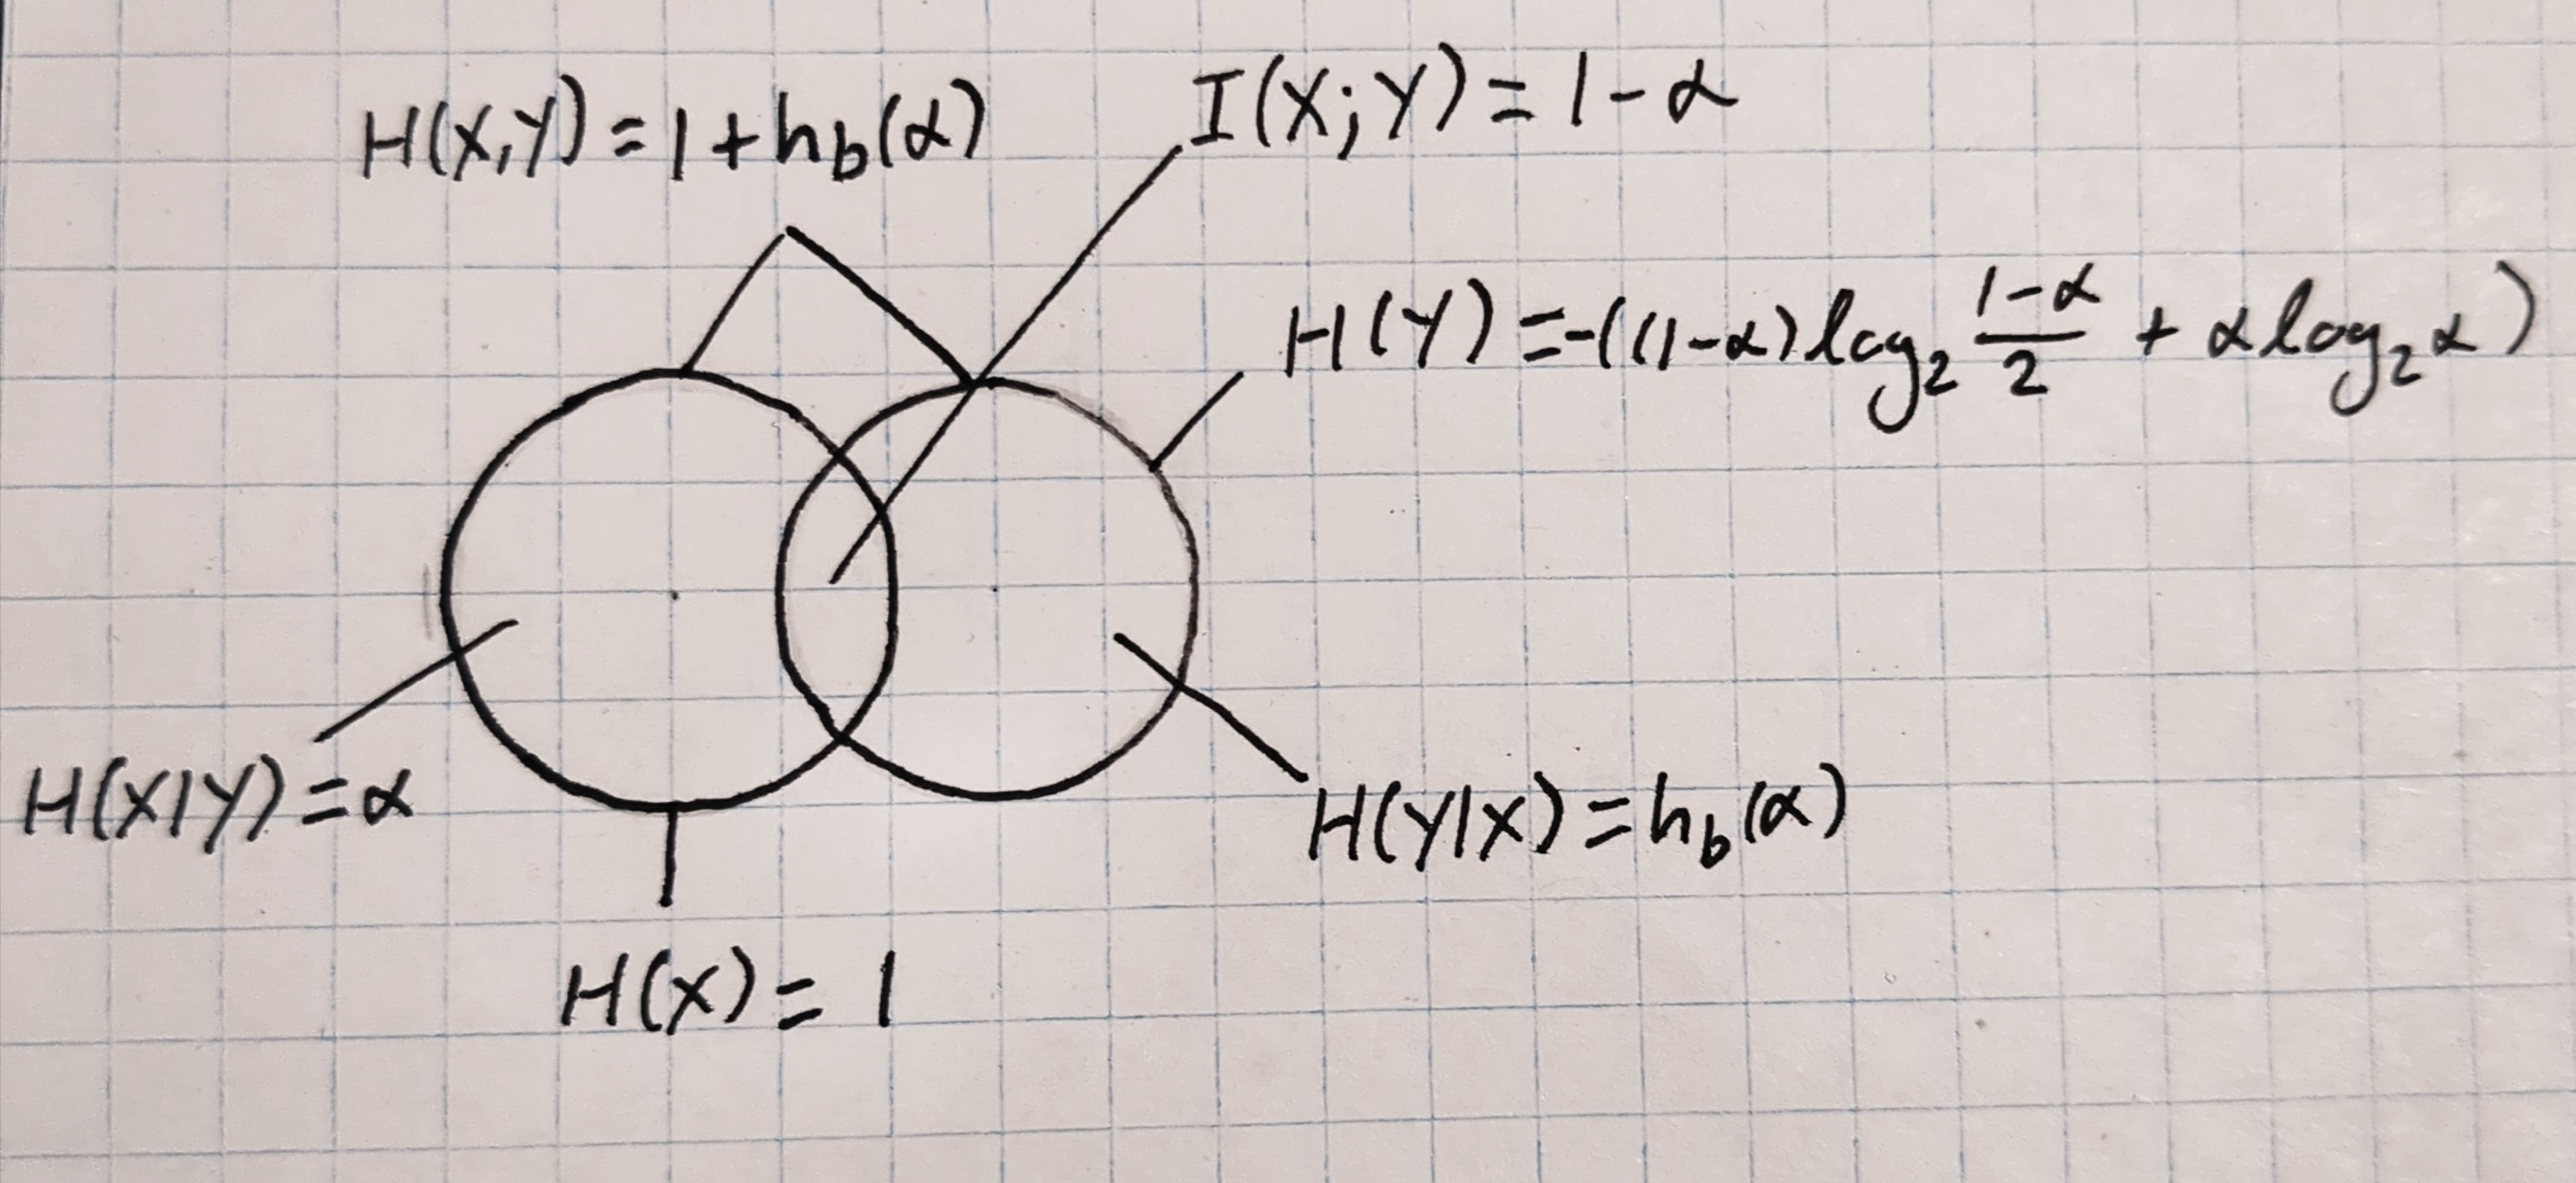
\includegraphics[width=130mm]{entropy-venn.jpg}}
\end{center}
{\bf Figure 1} Venn diagram depicting the relationships between the conditional, marginal and joint entropies of discrete {\it r.v.}s $X$ and $Y$, along with
the mutual information between $X$ and $Y$, denoted $I(X;Y)$.
\end{document}
